\def\rmm#1{{\bf \sc Robert: }{\marrow\sf #1}}


\subsection{Pre-processing} \label{subsec:preprocessing}

\begin{table}
	\caption{Overview of the pre-processing methods used in \ac{cad} systems.}
	\small
	%\renewcommand{\arraystretch}{1.5}
	\begin{tabular}{p{.65\linewidth} p{.25\linewidth}}
		\hline \\ [-1.5ex]
		\textbf{Pre-processing operations} & \textbf{References} \\ \\ [-1.5ex]
		\hline \\ [-1.5ex]
		\textit{\ac{mri} pre-processing:} & \\ \\ [-1.5ex]
		\quad Noise filtering: &  \\
		\quad \quad Median filtering & $[$20-21$]$  \\
		\quad \quad Wavelet-based filtering & $[$1-2,14$]$ \\ \\ [-1.5ex]
		\quad Bias correction: & \\
		\quad \quad Parametric methods & $[$15-35$]$ \\
		\quad \quad Non-parametric methods & $[$36$]$ \\ \\ [-1.5ex]
		\quad Standardization: & \\
		\quad \quad Statistical-based normalization: & $[$3-4,15,20-21,35,37$]$ \\
		\quad \quad Organ \ac{si}-based normalization & $[$18-19$]$ \\ \\ [-1.5ex]
		\textit{\ac{mrsi} pre-processing:} & \\ \\ [-1.5ex]
		\quad Phase correction & $[$22$]$ \\
		\quad Water and lipid residuals filtering & $[$8$]$ \\
		\quad Baseline correction & $[$22,31$]$ \\
		\quad Frequency alignment & $[$31$]$ \\
		\quad Normalization & $[$22$]$ \\ \\ [-1.5ex]
		\hline
	\end{tabular}
\end{table}

\subsubsection{\ac{mri} images pre-processing}

Three different groups of pre-processing methods are commonly applied to images as initial stage in \ac{cad}.

\setenumerate{listparindent=\parindent,itemsep=10px}
\setlist{noitemsep}
\begin{enumerate}[leftmargin=*]

\begin{figure}
\centering
	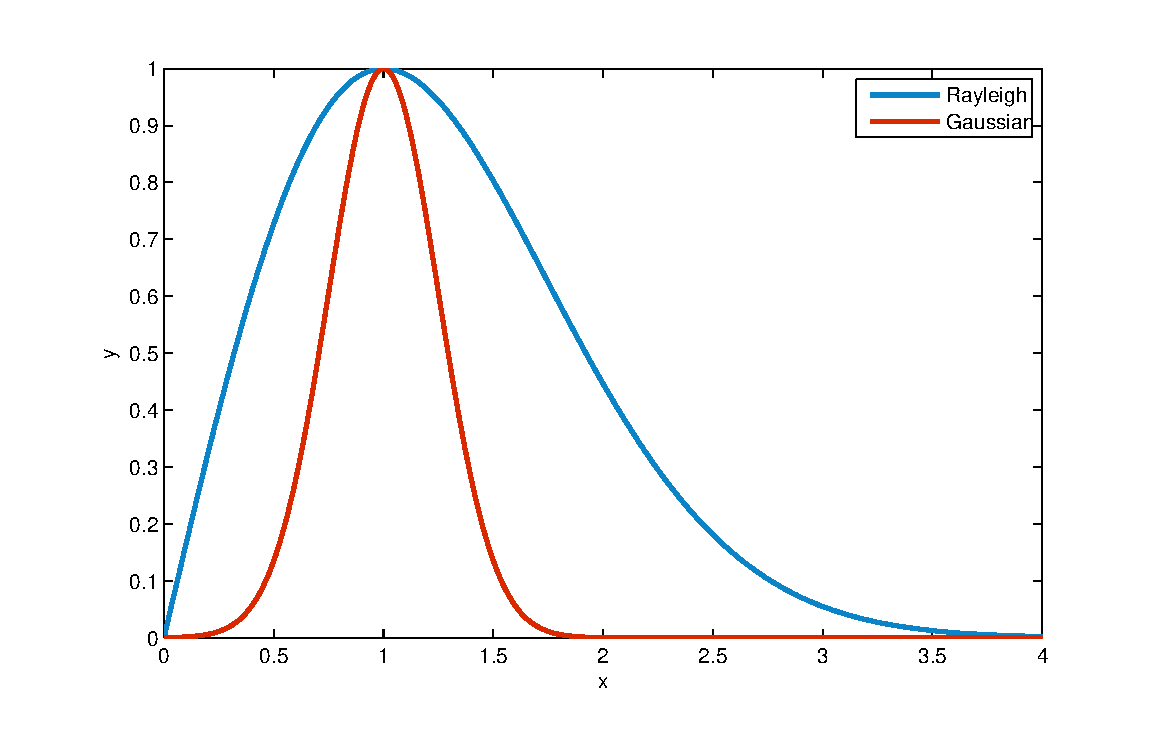
\includegraphics[width=0.9\linewidth]{03_image_processing/03_preprocessing/figures/noise/noisedistr.eps}
	\caption{Illustration of a Gaussian distribution ($\mu = 1, \sigma=0.25$) and a Rayleigh distribution ( $\sigma = 2$). It can be seen that the Rayleigh distribution is suffering of a bias term when compared with the Gaussian distribution.}
	\label{fig:noisedistr}
\end{figure}

%Noise filtering
\item[$-$] \textbf{\textit{Noise filtering:}} The \ac{nmr} signal measured and recorded in the k-space during an \ac{mri} acquisition is affected by noise. This noise obeys a complex Gaussian white noise mainly due to thermal noises in the patient area (\cite{Nowak1999}). Furthermore, \ac{mri} images visualized by radiologists are in fact the magnitude images resulting from the complex Fourier transform of the k-space data. The complex Fourier transform, being a linear and orthogonal transform, does not affect the Gaussian noise characteristics (\cite{Nowak1999}). However, the function involved in the magnitude computation is a non-linear transform (i.e., the square root of the sum of squares of real and the imaginary parts), implying that the noise distribution is no longer Gaussian; it indeed follows a Rician distribution making the denoising task harder. Briefly, a Rician distribution can be characterized as follows: in low-\ac{si} region (low \ac{snr}), it can be approximated with a Rayleigh distribution while in high-\ac{si} region (high \ac{snr}), it is similar to a Gaussian distribution (see Fig. \ref{fig:noisedistr}) (\cite{Manjon2008}). Reviews of all denoising methods can be found in the work of \cite{Buades2005} and \cite{Mohan2014}.

Median filtering is the simplest approach used to address the denoising issue in \ac{mri} images (\cite{Ozer2009,Ozer2010}). In both studies, Ozer et al. used a square kernel of size $5 \times 5$ pixels with the image resolutions ranging from $320 \times 256$ (cf., \ac{t2w} \ac{mri}) to $256 \times 128$ (cf., T$_2$ map, \ac{dce} and \ac{dw} \ac{mri}) and \iac{fov} ranging from 14 cm (cf, \ac{t2w} and \ac{dw} \ac{mri}) to 20 cm (cf, T$_2$ map and \ac{dce} \ac{mri}). However, from a theoretical point of view, this simple filtering method is not well formalized to address the noise distribution in \ac{mri} images.

More complex approaches were proposed to overcome this problem. A common method used to denoise \ac{mri} images is based on wavelet-based filtering. This filtering exploits the sparsity property of the wavelet decomposition. The projection of a noisy signal from the spatial-domain to the wavelet-domain implies that only few wavelet coefficients contribute to the ``signal-free noise'' while all wavelet coefficients contribute to the noise (\cite{Donoho1994}). Therefore, denoising is performed by thresholding/attenuating the insignificant wavelet coefficients to enforce the sparsity in the wavelet-domain. Investigations focus on the strategies to perform the most adequate coefficient shrinkage method (e.g., using thresholding, singularity property or Bayesian framework) (\cite{Pizurica2002}).

\cite{Ampeliotis2007,Ampeliotis2008} performed wavelet shrinkage to denoise magnitude \ac{mri} images (cf., \ac{t2w}-\ac{mri} and \ac{dce}-\ac{mri}) using thresholding techniques (\cite{Mallat2008}). However, since the wavelet transform is an orthogonal transform, the Rician distribution of the noise is preserved in the wavelet-domain. Hence, for low \ac{snr}, the wavelet and scaling coefficients still suffer from a bias due to this specific noise distribution (\cite{Nowak1999}). 

\cite{Lopes2011} used a technique proposed by \cite{Pizurica2003} to denoise \ac{t2w}-\ac{mri}. \cite{Pizurica2003} proposed a filtering technique based on joint detection and estimation theory (\cite{Middleton1968}). The wavelet coefficients ``free-of-noise'' are estimated from the noisy wavelet coefficients using a \ac{map} estimate. Furthermore, the estimator designed takes spatial context into account by including both local and global information in the prior probabilities. The different probabilities needed by the \ac{map} are empirically estimated by using mask images representing the locations of the significant wavelet coefficients. These mask images are computed by thresholding the detail images obtained from the wavelet decomposition. To remove the bias from the wavelet and scaling coefficients, the squared magnitude \ac{mri} image used instead of the magnitude \ac{mri} image as proposed by \cite{Nowak1999}. This involves changing the Rician distribution to a scaled non-central Chi-square distribution. It implies that the wavelet coefficients are also unbiased estimators and the scaling coefficients are unbiased estimators but up to a constant $C$ as defined in Eq. \eqref{eq:nowakC} which needs to be subtracted from each scaling coefficient,

\begin{equation}
	C=2^{(J+1)}\hat{\sigma}^2 \ ,
	\label{eq:nowakC}
\end{equation}

\noindent where $J$ is the number of levels of the wavelet decomposition and $\hat{\sigma}$ is an estimate of the noise standard deviation.

\begin{figure}
\centering
	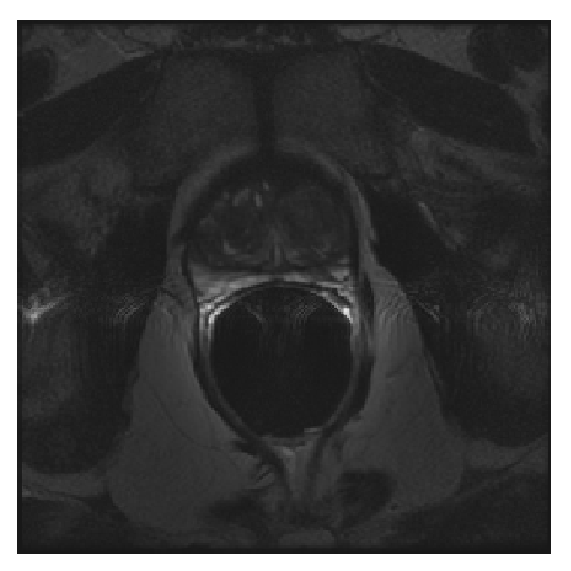
\includegraphics[width=0.5\linewidth]{03_image_processing/03_preprocessing/figures/bias/t2w_bias_antenna.eps}
	\caption{Example of artefacts with high \ac{si} due to perturbation from the endorectal coil which create inhomogeneity.}
	\label{fig:bias}
\end{figure}

% Artefacts filtering
\item[$-$] \textbf{\textit{Bias correction:}} Besides being corrupted by noise, \ac{mri} images are also affected by the inhomogeneity of the \ac{mri} field commonly referred to as bias field (\cite{Styner2000}). This bias field results in a smooth variation of the \ac{si} through the image. When an endorectal coil is used, an artefact resulting of an hyper-intense signal can be observed around the coil on the images (see Fig. \ref{fig:bias}). As a consequence, the \ac{si} of identical tissues varies depending on their spatial location in the image making further processes such as segmentation or registration harder (\cite{Jungke1987,Vovk2007}). A review of bias correction methods can be found in \cite{Vovk2007}.

The model of image formation is usually formalized such that:

\begin{equation}
	ss(\mathbf{x}) = o(\mathbf{x})b(\mathbf{x}) + \eta(\mathbf{x}) \ ,
	\label{eq:biasmodel}
\end{equation}

\noindent where $s(\mathbf{x})$ is the corrupted \ac{si} at the pixel for the image coordinates $\mathbf{x} = \{x,y\}$, $o(\mathbf{x})$ is the ``noise-free signal'' , $b(\mathbf{x})$ is the bias field function and $\eta(\mathbf{x})$ is an additive white Gaussian noise.
%
%By using property of logarithm, the model of Eq. \eqref{eq:biasmodel} becomes additive such that:
%
%\begin{eqnarray}
%	\log s(\mathbf{x}) - \log b(\mathbf{x}) & = & \log \left( o(\mathbf{x}) + \frac{\eta(\mathbf{x})}{b(\mathbf{x})} \right) \ , \\ \nonumber
%	& = & \log \hat{o}(x) \ .
%\end{eqnarray}
%
%\noindent where $\hat{o}(\mathbf{x})$ is the signal only degraded by noise \cite{Styner2000}.

Hence, the task of bias correction involves estimating the bias function $b(\mathbf{x})$ in order to infer the ``signal-free bias'' $o(\mathbf{x})$.% and subtract to the logarithm of the initial signal in order to obtain an estimated ``signal-free bias''.

\cite{Viswanath2009} performed bias correction on \ac{t2w}-\ac{mri} using a parametric Legendre polynomial model proposed by \cite{Styner2000} and available in the \ac{itk} library\footnote{The \ac{itk} library is available at: \texttt{http://www.itk.org/}}. \cite{Styner2000} chose to model the bias field by using a linear combination of Legendre polynomials as:

\begin{equation}
	\hat{b}(\mathbf{x},\mathbf{p}) = \sum_{i=0}^{m-1} p_i f_i(\mathbf{x}) =  \sum_{i=0}^{l} \sum_{j=0}^{l-i} p_{ij} P_i(x) P_j(y) \ ,
	\label{eq:biascorr}
\end{equation}

\noindent where $\hat{b}$ is the bias estimation with the image coordinates $\mathbf{x} = \{x,y\}$ and the $m$ coefficients of the linear combination $\mathbf{p} = {p_{11},\dotsc,p_{ij}}$ ; $m$ can be defined as $m=(l+1)\frac{(l+2)}{2}$ where $l$ is the degree of Legendre polynomials chosen and $P_i(\cdot)$ denotes a Legendre polynomial of degree $i$.

This family of functions allows us to model the bias as a smooth inhomogeneity function across the image. To estimate the set of parameters $\mathbf{p}$, a cost function is defined which relies on the following assumptions: (i) an image is composed of $k$ regions with $\mu_k$ being the mean \ac{si} and a variance $\sigma^{2}_{k}$ of each particular class, and (ii) each noisy pixel belongs to one of the $k$ regions with its \ac{si} value close to the class mean $\mu_k$. Hence, the cost function is defined as:

\begin{equation}
	C(\mathbf{p}) = \sum_{\mathbf{x}} \prod_{k} \rho_k(s(\mathbf{x}) - \hat{b}(\mathbf{x},\mathbf{p}) - \mu_k) \ ,
	\label{eq:costbias}
\end{equation}

\begin{equation}
	\rho_k(x) = \frac{x^2}{x^2 + 3 \sigma_k^2} \ ,
	\label{eq:mestbias}
\end{equation}

\noindent where $\rho_k(\cdot)$ is a M-estimator allowing estimations to be less sensitive to outliers than usual square distance (\cite{Li1996}).

Finally, estimation of the parameters $\mathbf{p}$ results in finding the minimum of the cost function $C(\mathbf{p})$. This optimization was performed using the non-linear $(1+1)$ \ac{es} optimizer (\cite{Styner1997}).

In a later publication, \cite{Viswanath2012} make use of the well known N3 algorithm\footnote{The N3 algorithm implementation is available at: \texttt{http://www.bic.mni.\allowbreak mcgill.ca/software/N3/}} to correct \ac{t2w}-\ac{mri} developed by \cite{Sled1998}. To estimate the bias function, \cite{Sled1998} proposed to estimate the \acp{pdf} of the signal and bias.

Recalling Eq. \eqref{eq:biasmodel} and taking advantage of logarithm property, it implies that this model becomes additive such that:

\begin{eqnarray}
	\log s(\mathbf{x}) & = & \log b(\mathbf{x}) + \log \left( o(\mathbf{x}) + \frac{\eta(\mathbf{x})}{b(\mathbf{x})} \right) \ , \nonumber \\
	& \approx & \log b(\mathbf{x}) + \log \hat{o}(\mathbf{x}) \ , \label{eq:logbias}
\end{eqnarray}

\noindent where $\hat{o}(\mathbf{x})$ is the signal only degraded by noise. \cite{Sled1998} shows that Eq. \eqref{eq:logbias} can be related to \acp{pdf} such that:

\begin{equation}
	S(s) = B(s) * O(s) \ ,
	\label{eq:distrbias} 
\end{equation}

\noindent where $S$, $B$ and $O$ are respectively the probability densities of $s$, $b$ and $o$.

Restoring the corrupted signal $s$ is carried out by finding the multiplicative field $b$ which maximizes the frequency content of the distribution $O$. \cite{Sled1998} argue that a search through all possible fields $b$ and selection of the one which maximizes the high frequency content of $O$ could be carried out but results in an exhaustive search. However, they show that the bias field distribution can be assimilated to a near Gaussian distribution. Using this fact as \textit{a priori}, it is then possible to infer the distribution $O$ using Wiener deconvolution given $B$ and $S$ and later estimate the corresponding smooth field $b$.

\cite{Lv2009} corrected the inhomogeneity in \ac{t2w}-\ac{mri} images by using the method proposed by \cite{Madabhushi2006}. In this method, the \ac{mri} images are corrected iteratively by successively detecting the image foreground via \ac{gscale} and estimating a bias field function based on a second-order polynomial model. First the background of the \ac{mri} image is eliminated by threholding. The threshold value is commonly equal to the mean \ac{si} of the considered image. Then, in the seeded region growing algorithm is applied considering every thresholded pixel as a potential seed. However, pixels already assigned to a region will not be considered any more as seed. As in seeded region growing algorithm (\cite{Shapiro2001}), two criteria are taken into account to expand the region. First, the region will grow using a connected-neighbourhood, initially defined by the user. Then, the homogeneity of \ac{si} is based on a fuzzy membership function taking into account the absolute difference of the \acp{si} of two pixels. Depending on the membership value (cf., a threshold has to be defined), the pixel considered is merged or not to the region. Once this segmentation is performed, the largest region $R$ is used as a mask to select pixels of the original image and the mean \ac{si}, $\mu_{R}$, is computed. The background variation $b(\mathbf{x})$ is estimated as:

\begin{equation}
	b(\mathbf{x}) = \frac{s(\mathbf{x})}{\mu_{R}}, \ \forall \mathbf{x} \in R \ ,
	\label{eq:backest}
\end{equation}

\noindent where $s(\mathbf{x})$ is the original \ac{mri} image.

Finally, a second order polynomial $\hat{b}_{\Theta}(\mathbf{x})$ is fitted in a least-squares sense (Eq. \eqref{eq:lsolv}),

\begin{equation}
	\hat{\Theta} = \argmin_{\Theta} | b(\mathbf{x}) - \hat{b}_{\Theta}(\mathbf{x}) |^{2}, \ \forall \mathbf{x} \in R \ .
	\label{eq:lsolv}
\end{equation}

Finally, the whole original \ac{mri} image is corrected by dividing it by the estimated bias field function $\hat{b}_{\Theta}(\mathbf{x})$. This process is repeated until the number of pixels in the largest region $R$ does not change significantly between two iterations.

%SI normalization
\item[$-$] \textbf{\textit{\Ac{si} normalization/standardization:}}

As discussed in the later section, segmentation or classification tasks are usually performed by first learning from a training set of patients. Hence, one can emphasize the desire to perform \ac{mri} examinations with a high repeatability or in other words, one would ensure to obtain similar \ac{mri} images (cf., similar \acp{si}) for patients of the same group (cf., healthy patients \textit{vs.} patients with \ac{cap}), for a similar sequence.

However, it is a known fact that variability between patients occurs during the \ac{mri} examinations even using the same scanner, protocol or sequence parameters (\cite{Nyul1999}). Hence, the aim of normalization or standardization of the \ac{mri} data is to remove the variability between patients and enforce the repeatability of the \ac{mri} examinations.

Approaches used to standardize \ac{mri} images can be either categorized as statistical-based standardization or organ \ac{si}-based standardization. 

\cite{Artan2009,Artan2010} as well as \cite{Ozer2009,Ozer2010} standardized \ac{t2w}, \ac{dce} and \ac{dw} \ac{mri} images by computing the \textit{standard score} (also called \textit{z-score}) of the pixels of the \ac{pz} as:

\begin{equation}
	I_s(\mathbf{x}) = \frac{ I_r(\mathbf{x}) - \mu_{pz}}{\sigma_{pz}}, \ \forall \mathbf{x} \in \text{PZ} \ ,
	\label{eq:meansta}
\end{equation}

\noindent where $I_s(\mathbf{x})$ is the standardized \ac{si} with the image coordinates $\mathbf{x} = \{x,y\}$, $I_r(\mathbf{x})$ is the raw \ac{si}, $mu_{pz}$ is the mean-\ac{si} of the \ac{pz} and $\sigma_{pz}$ is the \ac{si} standard deviation in the \ac{pz}.

This transformation enforces the image \ac{pdf} to have a zero mean and a unit standard deviation. In a similar way, \cite{Liu2013} normalized \ac{t2w}-\ac{mri} by making use of the median and interquartile range for all the pixels.

\begin{equation}
	I_s(\mathbf{x}) = \frac{ I_r(\mathbf{x}) - Q_2}{Q_3 - Q_1}, \ \forall \mathbf{x} \ ,
	\label{eq:medsta}
\end{equation}

\noindent where $I_s(\mathbf{x})$ is the standardized \ac{si} with the images coordinates $\mathbf{x} = \{x,y\}$, $I_r(\mathbf{x})$ is the raw \ac{si} and with $Q_1$, $Q_2$ and $Q_3$ being respectively the first quartile, the median and the third quartile respectively.

\cite{Lv2009} scaled the \ac{si} of \ac{t2w}-\ac{mri} images using the method proposed by \cite{Nyul2000} based on \ac{pdf} matching. This approach is based on the assumption that \ac{mri} images from the same sequence should share the same \ac{pdf} appearance. Hence, one can approach this issue by transforming and matching the \acp{pdf} using some statistical landmarks such as median and different quantiles. Using a training set, these statistical landmarks are extracted for $N$ training images as for instance for the minimum, the $25^{\text{th}}$ quantile, the median, the $75^{\text{th}}$ quantile and the maximum:

\begin{eqnarray}	
	\Phi_{0} & = & \{ \phi_{0}^{1}, \phi_{0}^{2}, \cdots, \phi_{0}^{N} \} \ , \nonumber \\
	\Phi_{25} & = & \{ \phi_{25}^{1}, \phi_{25}^{2}, \cdots, \phi_{25}^{N} \} \ , \nonumber \\
	\Phi_{50} & = & \{ \phi_{50}^{1}, \phi_{50}^{2}, \cdots, \phi_{50}^{N} \} \ ,  \label{eq:quantileStd} \\
	\Phi_{75} & = & \{ \phi_{75}^{1}, \phi_{75}^{2}, \cdots, \phi_{75}^{N} \} \ , \nonumber \\
	\Phi_{100} & = & \{ \phi_{100}^{1}, \phi_{100}^{2}, \cdots, \phi_{100}^{N} \} \ , \nonumber
\end{eqnarray}

\noindent where $\phi_{n^\text{th}}^{i^{\text{th}}}$ is the $n^{\text{th}}$ quantile of the $i^{\text{th}}$ training image.

\begin{figure}
	\centering
	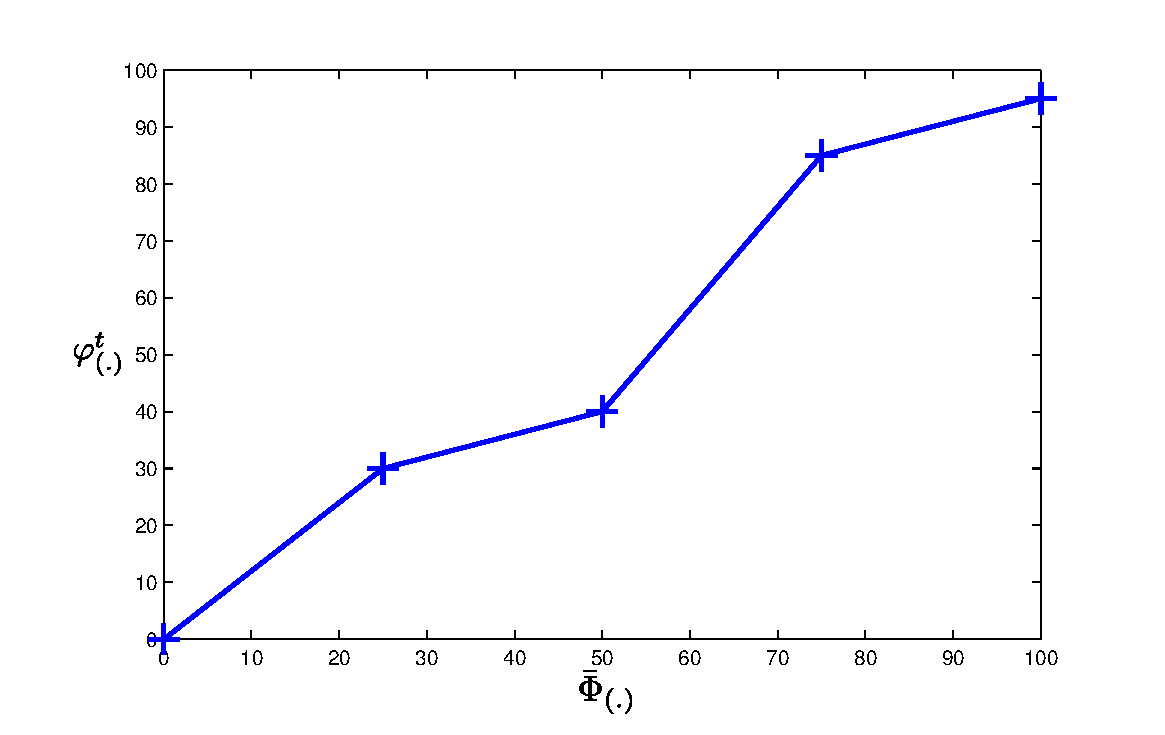
\includegraphics[width=0.9\linewidth]{03_image_processing/03_preprocessing/figures/normalization/linear_transform_parts.eps}
	\caption{Example of linear mapping by parts as proposed by \cite{Nyul2000}.}
	\label{fig:imnorm}
\end{figure}

Then, the mean of each quantile $\{ \bar{\Phi}_{0}, \bar{\Phi}_{25}, \bar{\Phi}_{50}, \bar{\Phi}_{75}, \bar{\Phi}_{100} \}$ is also calculated.
Once this training stage is performed, a linear transformation by parts $\mathcal{T}(\cdot)$ can be computed (Eq. \eqref{eq:linearMap}) for each test image $t$ by mapping each statistical landmark $\varphi_{(cdot)}̂^{t}$ of this image with the pre-learned statistical landmarks $\bar{\Phi}_{(\cdot)}$. This linear mapping is also depicted in Fig. \ref{fig:imnorm}.

\begin{equation}
\small
\mathcal{T}(s(\mathbf{x})) =
  \begin{cases}
    \lceil \bar{\Phi}_{0}+( s(\mathbf{x}) - \varphi_{0}^{t} ) \left( \frac{\bar{\Phi}_{25} - \bar{\Phi}_{0}}{\varphi_{25}^{t} - \varphi_{0}^{t}} \right) \rceil \ , & \text{if $\varphi_{0}^{t} \leq s(\mathbf{x})<\varphi_{25}^{t})$} \ , \\
    \lceil \bar{\Phi}_{25}+( s(\mathbf{x}) - \varphi_{25}^{t} ) \left( \frac{\bar{\Phi}_{50} - \bar{\Phi}_{25}}{\varphi_{50}^{t} - \varphi_{25}^{t}} \right) \rceil \ , & \text{if $\varphi_{25}^{t} \leq s(\mathbf{x})<\varphi_{50}^{t})$} \ , \\
    \lceil \bar{\Phi}_{50}+( s(\mathbf{x}) - \varphi_{50}^{t} ) \left( \frac{\bar{\Phi}_{75} - \bar{\Phi}_{50}}{\varphi_{75}^{t} - \varphi_{50}^{t}} \right) \rceil \ , & \text{if $\varphi_{50}^{t} \leq s(\mathbf{x})<\varphi_{75}^{t})$} \ , \\
   \lceil \bar{\Phi}_{75}+( s(\mathbf{x}) - \varphi_{75}^{t} ) \left( \frac{\bar{\Phi}_{100} - \bar{\Phi}_{75}}{\varphi_{100}^{t} - \varphi_{75}^{t}} \right) \rceil \ , & \text{if $\varphi_{75}^{t} \leq s(\mathbf{x})\leq \varphi_{100}^{t})$} \ ,
  \end{cases}
  \label{eq:linearMap}
\end{equation}

\cite{Viswanath2009,Viswanath2011,Viswanath2012} use a variant of this previous approach presented in the work of \cite{Madabhushi2006a} aiming to standardize the \ac{t2w}-\ac{mri} images. Instead of computing the \ac{pdf} of an entire image, a pre-segmentation of the foreground is carried out via \ac{gscale} which was discussed in the bias correction section. Once the foreground is detected, the largest region is extracted and the same process than previously mentioned (see Eq. \eqref{eq:linearMap}) takes place in order to align \acp{pdf} of the foreground of the \ac{mri} images.

\begin{figure}
\centering
	\hspace*{\fill}
	\subfigure[Illustration and location of the bladder on a \ac{t2w}-\ac{mri} image acquired with a 3.0 Tesla \ac{mri} scanner]{\label{subfig:bladder} 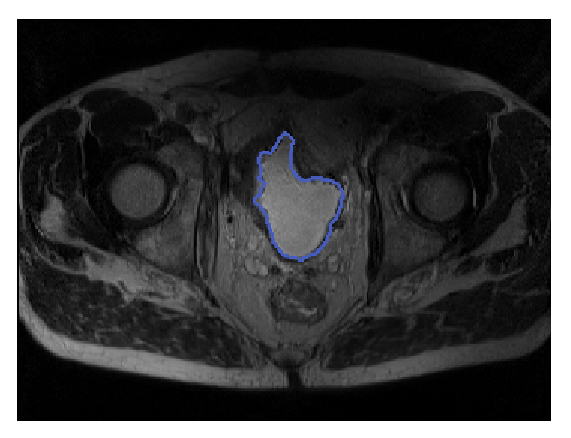
\includegraphics[width=0.45\linewidth]{03_image_processing/03_preprocessing/figures/niaf/t2w_bladder.eps}} \hfill
	\subfigure[Illustration and location of the femoral arteries on a \ac{t1w}-\ac{mri} image acquired with a 3.0 Tesla \ac{mri} scanner]{\label{subfig:arteries} 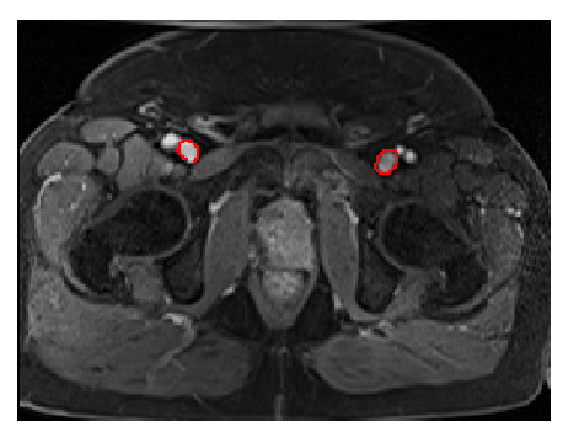
\includegraphics[width=0.45\linewidth]{03_image_processing/03_preprocessing/figures/niaf/t1w_arteries.eps}}
	\hspace*{\fill}
	\caption{Illustration of the two organs used by \cite{Niaf2011,Niaf2012} to normalize \ac{t2w} and \ac{t1w} \ac{mri} images.}
	\label{fig:niaf}
\end{figure}

The methods described above were statistical-based methods. However, the standardization problem can be tackled by normalizing the MRI images using the \ac{si} of some known organs present in these images. \cite{Niaf2011,Niaf2012} normalized \ac{t2w}-\ac{mri} images by dividing the original \ac{si} of the images by the mean \ac{si} of the bladder (see Fig. \ref{subfig:bladder}). Likewise, \cite{Niaf2011} standardized the \ac{t1w}-\ac{mri} images using the \ac{aif}. They computed the \ac{aif} by taking the mean of the \ac{si} in the most enhanced part of the common femoral arteries (see Fig. \ref{subfig:arteries}) as proposed by \cite{Wiart2007}.

\end{enumerate}

\subsubsection{\ac{mrsi} spectra}

Presented in Sect. \ref{subsubsec:mrimrsi}, \ac{mrsi} is a modality related to a one dimensional signal. Hence, specific pre-processing steps for this type of signals have been applied instead of standard signal processing methods.

\setenumerate{listparindent=\parindent,itemsep=10px}
\setlist{noitemsep}
\begin{enumerate}[leftmargin=*]

	\item[$-$] \textbf{\textit{Phase correction:}} \ac{mrsi} data acquired suffer from zero-order and first-order phase misalignments as shown in Fig. \ref{fig:phase} (\cite{Chen2002,Osorio-Garcia2012}). 
	
\cite{Parfait2012} used a method proposed by \cite{Chen2002} where the phase of \ac{mrsi} signal is corrected based on entropy minimization in  the frequency domain. The corrected \ac{mrsi} signal $o(\xi)$ can be expressed as:

\begin{eqnarray}
	\Re(o(\xi)) & = & \Re(s(\xi))\cos(\Phi(\xi)) - \Im(\xi)\sin(\Phi(\xi)) \ , \nonumber  \\
	\Im(o(\xi)) & = & \Im(s(\xi))\cos(\Phi(\xi)) + \Re(\xi)\sin(\Phi(\xi)) \ , \nonumber \\
	\Phi(\xi) & = & \phi_0 + \phi_1 \frac{\xi}{N} \ , \label{eq:mrsiphcorr}
\end{eqnarray}

\noindent where $\Re(\cdot)$ and $\Im(\cdot)$ are the real and imaginary part of the complex signal respectively, $s(\xi)$ is the corrupted \ac{mrsi} signal, $\phi_0$ and $\phi_1$ are the zero-order and first-order phase correction terms respectively and $N$ is the total number of samples of the \ac{mrsi} signal.

\cite{Chen2002} tackled this problem using an optimization framework where $\phi_0$ and $\phi_1$ had to be inferred. Hence, the simplex Nelder-Mead optimization method was used to minimize the following cost function based on the Shannon entropy formulation:

\begin{equation}
	\hat{\Phi} = \argmin_{\Phi} \left[ - \sum \Re(s'(\xi)) \ln \Re(s'(\xi)) + \lambda \|\Re(s(\xi))\|_2 \right] \ ,
	\label{eq:phcost}
\end{equation}

\noindent where $s'(\xi)$ is the first derivative of the corrupted signal $s(\xi)$ and $\lambda$ is a regularization parameter.

Once the best parameter $\Phi$ is obtained, the \ac{mrsi} signal is corrected using Eq. \eqref{eq:mrsiphcorr}.

\begin{figure}
	\centering
	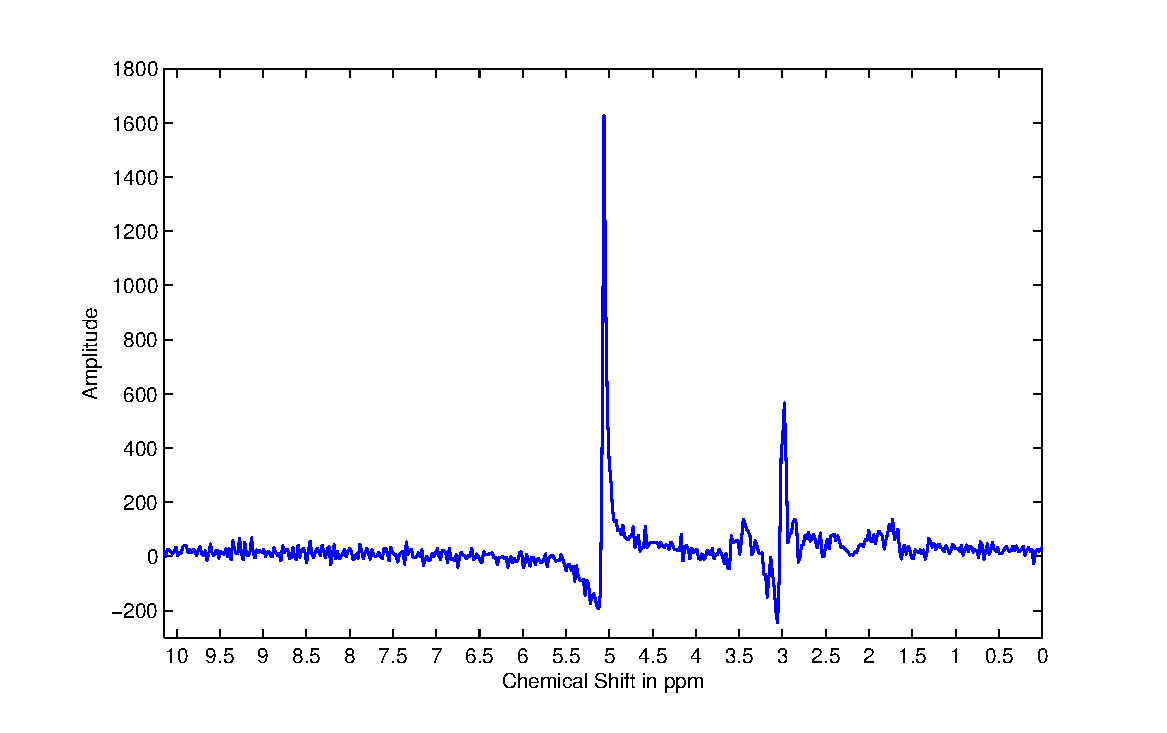
\includegraphics[width=0.9\linewidth]{03_image_processing/03_preprocessing/figures/phase/phase.eps}
	\caption{Illustration of phase misalignment in an \ac{mrsi} spectra acquire with a 3.0 Tesla \ac{mrsi} scanner. Note the distortion of the signal specially visible for the water and citrate peaks.}
	\label{fig:phase}
\end{figure}

	\item[$-$] \textbf{\textit{Water and lipid residuals filtering:}} The water and lipid metabolites occur in much higher concentrations the metabolites of interests (cf., choline, creatine and citrate) (\cite{Zhu2010,Osorio-Garcia2012}). Fortunately, specific \ac{mrsi} sequences were developed in order to suppress water and lipid metabolites using pre-saturation techniques (\cite{Zhu2010}). However, these techniques do not perfectly remove water and lipids peaks and some residuals are still present in the \ac{mrsi} spectra as shown in Fig. \ref{fig:waterfat}. Therefore, different post-processing methods have been proposed to enhance the quality of the \ac{mrsi} spectra by removing these residuals.
	
	\cite{Kelm2007} used the well known HSVD algorithm proposed by \cite{Pijnappel1992}. In the time domain, a \ac{mrsi} signal $s(t)$ is modelled by a sum of $K$ exponentially damped sinusoids such that:
\begin{equation}
	s(t) = \sum_{k=1}^{K} a_{k}\exp(i \phi_k) \exp( -d_{k} + i 2 \pi f_{k} ) t + \eta(t) \ ,
	\label{eq:fidsig}
\end{equation}

\noindent where $a_k$ is the amplitude proportional to the metabolite concentration with a resonance frequency $f_{k}$, $d_k$ represents the damping factor of the exponential, $\phi_k$ is the first-order phase and $\eta(t)$ is a complex white noise. 

\cite{Pijnappel1992} showed that the ``noise-free signal'' can be found using the \ac{svd} decomposition. First the noisy signal is reorganized inside a Hankel matrix $H$. It can be shown that if the signal considered would be a ``noise-free signal'', the rank of $H$ would be equal to rank $K$. However, due to the presence of noise, $H$ is in fact a full rank matrix. Thus, to recover the ``noise-free signal'', the rank of $H$ can be truncated to $K$ using its \ac{svd} decomposition. Hence, knowing the cut off frequencies of water (cf., 4.7 ppm) and lipid (cf., 2.2 ppm) metabolites, their corresponding peaks can be reconstructed and subtracted from the original signal (\cite{Laudadio2002}).

\begin{figure}
\centering
	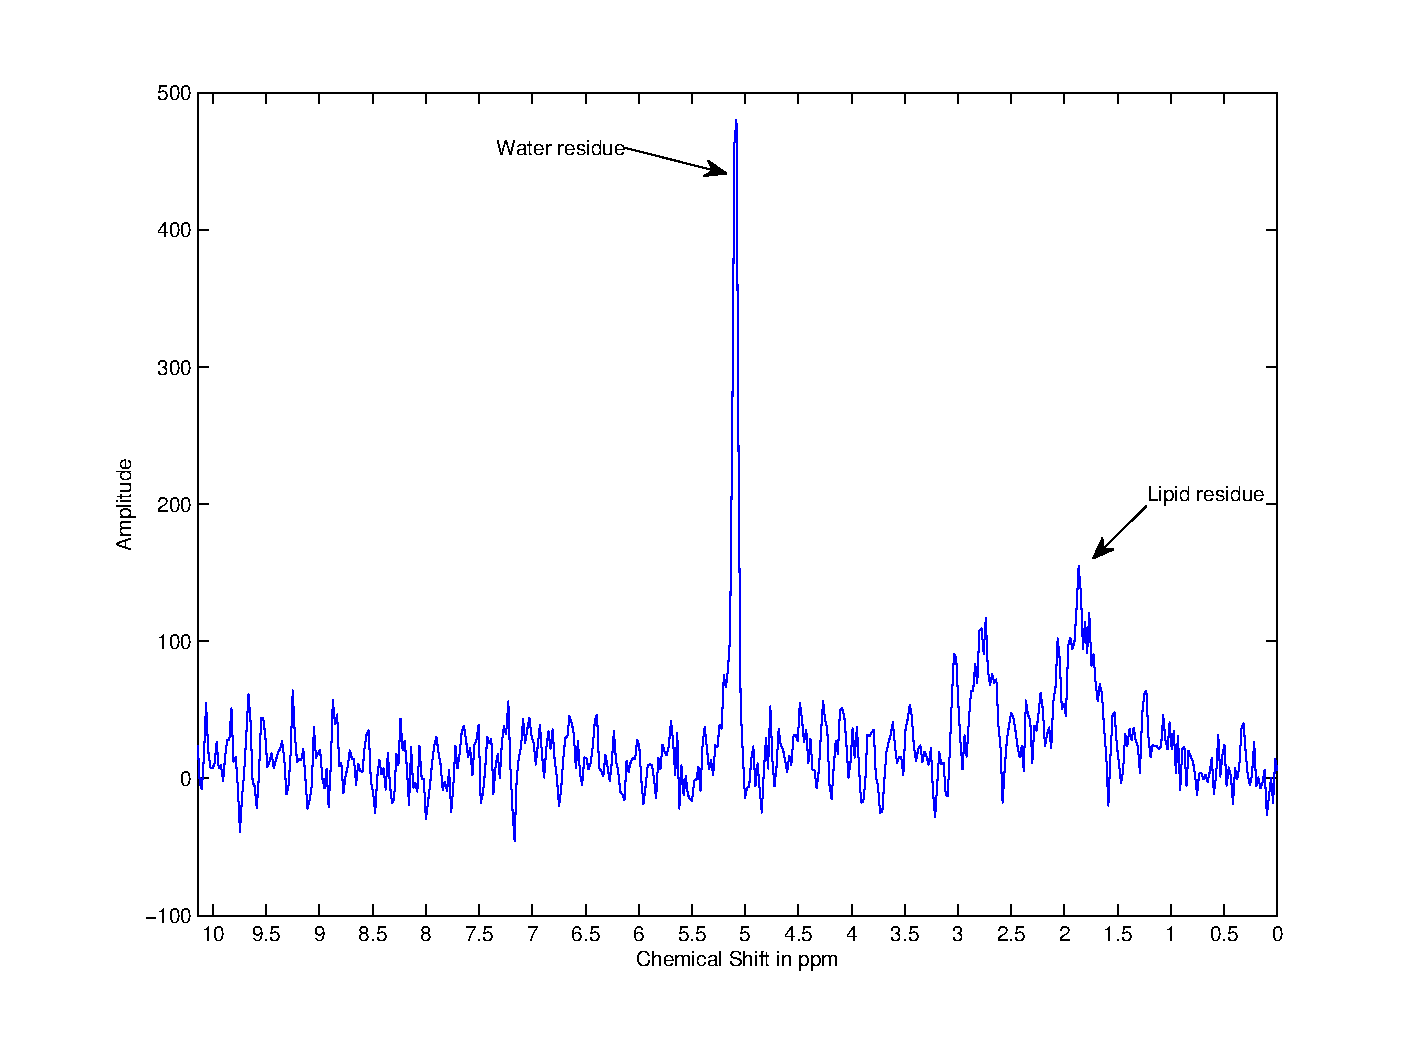
\includegraphics[width=0.9\linewidth]{03_image_processing/03_preprocessing/figures/water/water_fat.eps}
	\caption{Illustration of the residues of water and fat even after their suppression during the acquisition protocol. The acquisition was carried out with a 3.0 Tesla \ac{mri}.}
	\label{fig:waterfat}
\end{figure}
	
\item[$-$] \textbf{\textit{Baseline correction:}} Sometimes, the problem discussed in the above section regarding the lipid molecules is not addressed simultaneously with water residuals suppression. Lipids and macromolecules are known to affect the baseline of the \ac{mrsi} spectra. They could cause errors during further fitting processes aiming to quantify the metabolites, especially regarding the citrate metabolite.
	
\cite{Parfait2012} made the comparison of two different methods to detect the baseline and correct the \ac{mrsi} spectra which are based on the work of \cite{Lieber2003} and \cite{Devos2004}. \cite{Lieber2003} addressed the problem of baseline detection in the frequency domain by fitting a polynomial of low degree $p(x)$ (e.g., second or third degree) to the \ac{mrsi} signal $s(x)$ in a least-squares sense. Then, the values of the fitted polynomial are re-assigned as:

\begin{equation}
	p_f(x) = 
	\begin{cases}
		p(x) \ , & \text{if $p(x) \leq s(x)$} \ , \\
		s(x) \ , & \text{if $p(x) > s(x)$} \ . \\
	\end{cases}
	\label{eq:lieber}
\end{equation}

Finally, this procedure of fitting and re-assignment is iteratively repeated on $p_f(x)$ until a stopping criterion is reached. The final polynomial function can be subtracted from the original signal s(x) to correct it.

\cite{Parfait2012} modified this algorithm by convolving a Gaussian kernel to smooth the \ac{mrsi} signal instead of fitting a polynomial function, keeping the rest of the algorithm identical. 

Unlike \cite{Lieber2003}, \cite{Devos2004} proposed to correct the baseline in the time domain by multiplying the \ac{mrsi} signal by a decreasing exponential function as:
\begin{equation}
	c(t) = \exp (- \beta t) \ ,
	\label{eq:devos}
\end{equation}

\noindent Having a typical value for $\beta$ of 0.15.

However, \cite{Parfait2012} concluded that the method proposed by \cite{Lieber2003} outperforms the one of \cite{Devos2004}. In the contemporary work of \cite{Tiwari2012}, the authors detected the baseline using a local non-linear fitting method avoiding regions with significant peaks which were  detected using a experimentally parametrised signal-to-noise ratio (i.e. a value larger than 5 dB).

\begin{figure}
\centering
	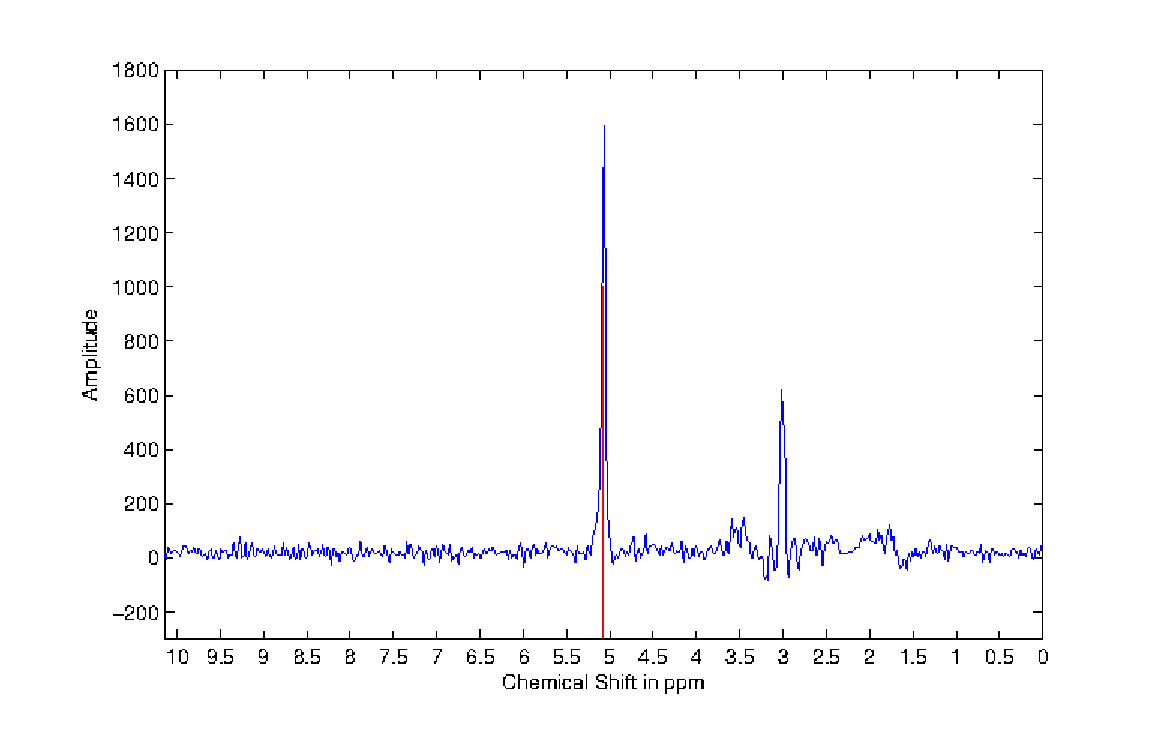
\includegraphics[width=0.9\linewidth]{03_image_processing/03_preprocessing/figures/frequency/frequency.eps}
	\caption{Illustration of frequency misalignment in an \ac{mrsi} spectra acquired with a 3.0 Tesla \ac{mrsi} scanner. The water peak is known to be aligned at 4.65 ppm. However, it can be seen that the peak on this spectra is aligned at around 5.1 ppm.}
	\label{fig:frequency}
\end{figure}

	\item[$-$] \textbf{\textit{Frequency alignment:}} Due to variations of the experimental conditions, a frequency shift can be observed in the \ac{mrsi} spectra as shown in Fig. \ref{fig:frequency} (\cite{Chen2002,Osorio-Garcia2012}).
	
\cite{Tiwari2012} corrected the frequency shift by first detecting known metabolite peaks such as choline, creatine and citrate. The frequency shift is corrected by minimizing the frequency error between the experimental and theoretical values of each of these peaks.

	\item[$-$] \textbf{\textit{Normalization:}} Due to variations of the experimental conditions, the \ac{mrsi} signal may also vary between patients.
	
\cite{Parfait2012} as \cite{Devos2004} compared two methods to normalize \ac{mrsi} signal. In each method, the original \ac{mrsi} spectra is divided by a normalization factor, similar to the intensity normalization described earlier. 

The first approach to obtain the normalization factor is based on an estimation of the water concentration. It is required to have an additional \ac{mrsi} sequence where the water metabolites are unsuppressed. Using this sequence, an estimation of the water concentration can be performed using the previously reported HSVD algorithm.  The second approach to normalization is based on using the L$_2$ norm of the \ac{mrsi} spectra $\|s(\xi)\|_2$. 
It should be noted that both \cite{Parfait2012} and \cite{Devos2004} concluded that the L$_2$ normalization was more efficient in their framework.
 
\end{enumerate}